%%%%%%%%%%%%%%%%%%%%%%%%%%%%%%%%%%%%%%%%%%%%%%%%%%%%%%%%%%%%%%%%%%%%
%% I, the copyright holder of this work, release this work into the
%% public domain. This applies worldwide. In some countries this may
%% not be legally possible; if so: I grant anyone the right to use
%% this work for any purpose, without any conditions, unless such
%% conditions are required by law.
%%%%%%%%%%%%%%%%%%%%%%%%%%%%%%%%%%%%%%%%%%%%%%%%%%%%%%%%%%%%%%%%%%%%

% This theme was based on fibeamer theme 
% If you found any bugs please contact @karlosos
% This repository is hosted on github https://github.com/karlosos/zut-fibeamer/

\documentclass{beamer}
\usetheme[faculty=wi]{fibeamer}
\usepackage[utf8]{inputenc}
\usepackage[
  main=polish,
  polish
]{babel}
\usepackage{hyperref}
\title{Aula 6  - Padrões}
\subtitle{Tópicos especiais em Sistemas}
\author{Prof. Juliana Costa Silva - juliana.silva@up.edu.br}

\usepackage{ragged2e}  % `\justifying` text
\usepackage{booktabs}  % Tables
\usepackage{tabularx}
\usepackage{tikz}      % Diagrams
\usetikzlibrary{calc, shapes, backgrounds}
\usepackage{amsmath, amssymb}
\usepackage{url}       % `\url`s
\usepackage{listings}  % Code listings
\frenchspacing
\begin{document}

%------------------------------------------------------------------------
  \frame[c]{\maketitle}
      \begin{frame}<beamer>
      \frametitle{O que veremos hoje}
      \tableofcontents
    \end{frame}
%------------------------------------------------------------------------
    \section{Revendo...}
    \begin{frame}{Revendo...}{O que já aprendemos?}
      
      \begin{itemize}
            \item Criamos um projeto node;
            \item Configuramos a porta do através do arquivo \textbf{index.js};
            \item Definimos rotas de get da nosso aplicação;
            \item Configuramos nodemon no ambiente dev;
       \end{itemize}
     \end{frame}
%------------------------------------------------------------------------
%    \begin{frame}[label=lists]{Ferramentas e tecnologias}
%      \begin{columns}[onlytextwidth]
%        \column{.5\textwidth}
%          \begin{itemize}
%            \item NodeJS \textcolor{gray}{(instalar até a próxima aula)}
%            \item VSCode \textcolor{gray}{(ou outra IDE da preferência do aluno)}
%            \item AngularJS 
%          \end{itemize}
%        \column{.5\textwidth}
%            
\includegraphics[width=55mm]{resources/aula1_4.png}
%      \end{columns}
%    \end{frame}
%------------------------------------------------------------------------
\begin{frame}[label=proof]{O projeto da disciplina}
	\begin{itemize}
	\item Faremos um sistema de controle financeiro pessoal;
	\item Este sistema deve ter:
	\begin{itemize}
	\item Registro de gastos;
	\item Login de usuários;
	\item Registro de renda (salários - comissões - negócios);
	\item Registro de cartões de créditos;
	\item Registro de contas bancárias;
	\end{itemize}
	\end{itemize}
    \end{frame}
%------------------------------------------------------------------------
\section{Introdução}
    \begin{frame}[label=lists]{Organização}
    \begin{exampleblock}{Qual a função do index.js?}
        	\begin{itemize}
	\item Inicia o servidor;
	\item Configura porta a escutar;
	\item Define rotas get de atendimentos e outras;
        	\end{itemize}
	\vspace{0.5cm}
	Falta organização ao projeto?
      \end{exampleblock}
    \end{frame}
%------------------------------------------------------------------------
\section{Pacotes/ módulos}
    \begin{frame}[label=lists]{Controller}

% \begin{columns}[onlytextwidth]
%        \column{.5\textwidth}
         Vamos criar a pasta \textbf{controller}.
         \begin{itemize}
         \item Esta pasta será responsável por organizar e gerenciar as ações da nossa aplicação. 
         \item Crie, dentro dessa pasta um arquivo chamado \textbf{movimento.js}, é nele que iremos controlar a rota app.get;
         \end{itemize}
          \vspace{0.5cm}
          Mova a \underline{linha 7} do arquivo \textbf{index.js}, conforme apresentado abaixo, para \textbf{movimento.js}.
%
%        \column{.5\textwidth}
	            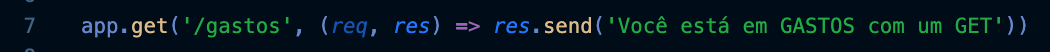
\includegraphics[width=110mm]{resources/aula4_1.png}\\
            \tiny{\textbf{Fonte:} O autor}
%      \end{columns}
    \end{frame}

 %------------------------------------------------------------------------
    \begin{frame}[label=lists]{Nova estrutura do Projeto }
    Crie a pasta controller:\\
    \begin{center}
    	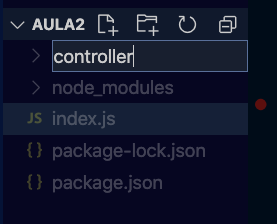
\includegraphics[width=70mm]{resources/aula4_2.png}\\
        \tiny{\textbf{Fonte:} O autor}
     \end{center}
    \end{frame}
    %------------------------------------------------------------------------
    \begin{frame}[label=lists]{Criando "Moviemnto.js" }
    Dentro da pasta controller, crie o arquivo movimento.js:\\

   \begin{columns}[onlytextwidth]
        \column{.5\textwidth}
    		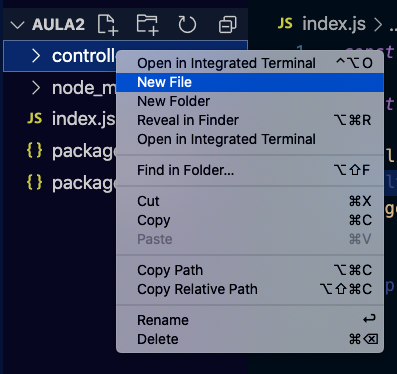
\includegraphics[width=50mm]{resources/aula4_3.png}\\
        		\tiny{Passo 1: clique com botão direito sobre a pasta controller e selecione "New File". \textbf{Fonte:} O autor}
         \column{.5\textwidth}
        		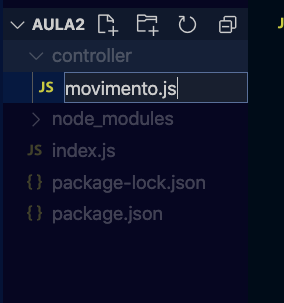
\includegraphics[width=50mm]{resources/aula4_4.png}\\
        		\tiny{Passo 2: Na caixa de diálogo digite o nome e a extensão do arquivo. \textbf{Fonte:} O autor}
       \end{columns}
    \end{frame}
     %------------------------------------------------------------------------
    \begin{frame}[label=lists]{Funciona?}
		\begin{exampleblock}{Importações necessárias}
	\begin{itemize}
	\item Se executar novamente o projeto, na rota movimento nada será exibido;
	\item Isto é, \textbf{movimentos.js} deixou de ser reconhecido;
	\item O que ocorreu porque não \underline{exportamos} este módulo (quando criamos arquivos separados, criamos módulos).
	\end{itemize}
	\end{exampleblock}
    \end{frame}
   
 %------------------------------------------------------------------------
 \section{Export}
    \begin{frame}[label=lists]{Export}
	\begin{exampleblock}{Exportando módulo}
		\begin{itemize}
			\item Essa função exporta o comando get configurado;
			\item Recebe por parâmetro \alert{app}.
		\end{itemize}
	\end{exampleblock}
	 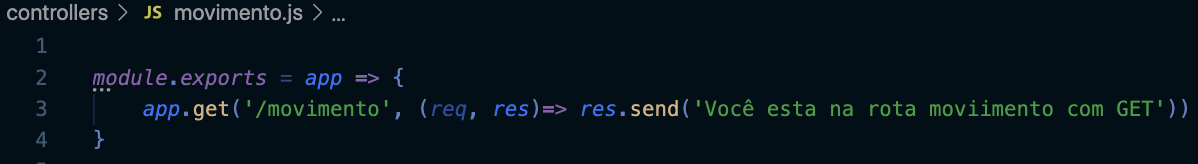
\includegraphics[width=105mm]{resources/aula4_6.png}\\
            \tiny{Função module.exports no arquivo movimento.js. \textbf{Fonte:} O autor}

    \end{frame}
   
    %------------------------------------------------------------------------
    \begin{frame}[label=lists]{Consign}
		\begin{exampleblock}{Para nos auxiliar nas exportações}
	\begin{itemize}
	\item Vamos instalar (via terminal) o consign, que vai agrupar todas as rotas e associa-las ao \alert{app}.
	\item Use o comando \alert{npm install consign} no terminal;
	\end{itemize}
	\end{exampleblock}
    \end{frame}
 %------------------------------------------------------------------------
    \begin{frame}[label=proof]{Controllers e app}
	\begin{itemize}
	\item Precisamos informar a aplicação que os arquivos de "controle" do nosso \alert{app}, ficarão reunidos na pasta \textbf{controllers}
	\item Para isso utilizaremos um objeto consign;
	\item Associaremos a ele todo o conteúdo da pasta \textbf{controllers} então nossa aplicação verá todas as rotas criadas por lá.
	\end{itemize}
	\begin{center}
    	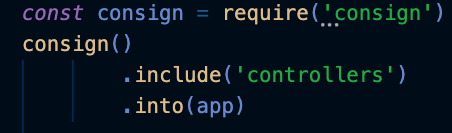
\includegraphics[width=70mm]{resources/aula4_7.png}\\
        \tiny{ Este código deve ser inserido no arquivo \textbf{index.js}, antes da utilização de \alert{app}. \textbf{Fonte:} O autor}
     \end{center}
    \end{frame}
 %------------------------------------------------------------------------
 \section{Módulo de configuração}
    \begin{frame}{Organizando [2]}
      %\begin{columns}[onlytextwidth]
        %\column{.5\textwidth}
	Nosso arquivo \textbf{index.js} ainda tem muitas funções....\\
	Será possível melhorar isso?
        
       % \column{.5\textwidth}
         \begin{center}
    	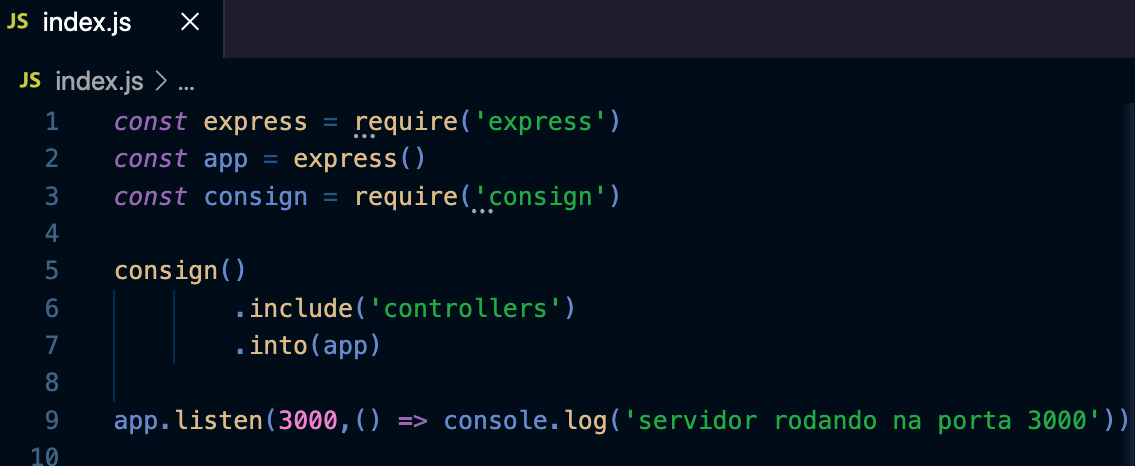
\includegraphics[width=110mm]{resources/aula4_8.png}\\
        \tiny{ Código no arquivo \textbf{index.js}. \textbf{Fonte:} O autor}
     \end{center}   
      % \end{columns}
    \end{frame}
    %------------------------------------------------------------------------
    \begin{frame}{Organizando [3]}
      %\begin{columns}[onlytextwidth]
        %\column{.5\textwidth}
	\begin{itemize}
		\item Crie uma pasta \textbf{config}, vamos separar todas as configurações do nosso app em um módulo;
		\item nessa pasta crie o arquivo \textbf{customExpress.js}.
		\item Recorte as linhas 1 a 7 do arquivo \textbf{index.js} e cole em \textbf{customExpress.js}.
		\item Essas linhas se referem a configuração da nossa aplicação;
	\end{itemize}
        
       % \column{.5\textwidth}
         \begin{center}
    	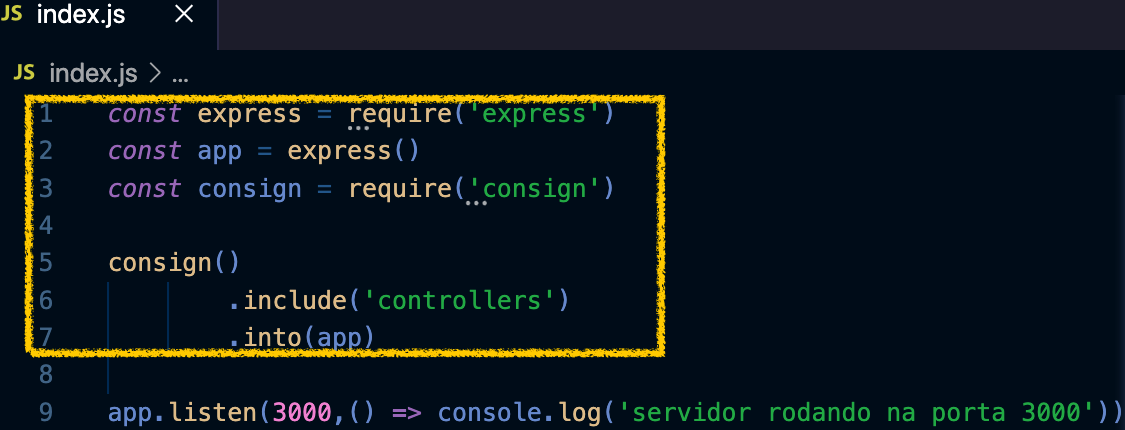
\includegraphics[width=100mm]{resources/aula4_9.png}\\
        \tiny{ Código no arquivo \textbf{index.js}. \textbf{Fonte:} O autor}
     \end{center}   
      % \end{columns}
    \end{frame}
%------------------------------------------------------------------------
    \begin{frame}{customExpress.js}
      %\begin{columns}[onlytextwidth]
        %\column{.5\textwidth}
 	Para garantir que o objeto \alert{app} exista no arquivo \textbf{index.js}, criaremos um \alert{module.export} e exportaremos a função, que retorna a variável app; 
        
       % \column{.5\textwidth}
         \begin{center}
    	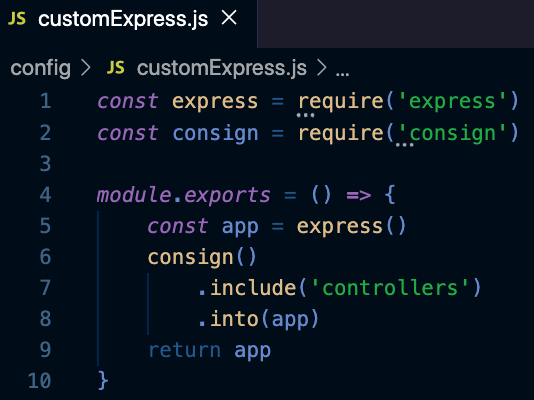
\includegraphics[width=75mm]{resources/aula4_10.png}\\
        \tiny{ Código no arquivo \textbf{customExpress.js}. \textbf{Fonte:} \cite{nodejs2022api}}
     \end{center}   
      % \end{columns}
    \end{frame}
    %------------------------------------------------------------------------
    \begin{frame}{Novo index.js}
      %\begin{columns}[onlytextwidth]
        %\column{.5\textwidth}
 	Agora, no index.js importaremos customExpress, ao invés de express.
        
       % \column{.5\textwidth}
         \begin{center}
    	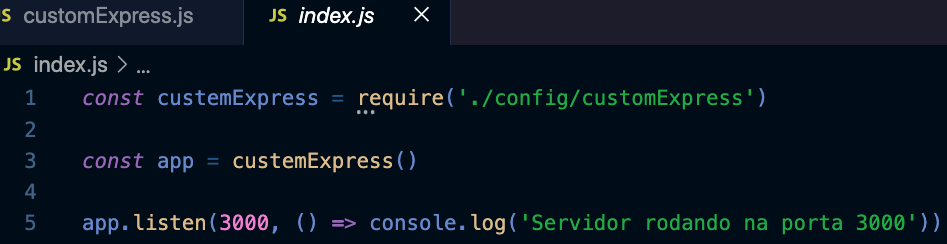
\includegraphics[width=110mm]{resources/aula4_11.png}\\
        \tiny{ Código no arquivo \textbf{index.js}. \textbf{Fonte:} O autor}
     \end{center}   
      % \end{columns}
    \end{frame}    

%------------------------------------------------------------------------
\section{Requisição POST}
 %------------------------------------------------------------------------
    \begin{frame}{movimentos.js}
      %\begin{columns}[onlytextwidth]
        %\column{.5\textwidth}
 	Em \textbf{movimentos.js}, como fazer para receber dados do usuário?\\
	Configuraremos o POST de nossa rota!
        
       % \column{.5\textwidth}
         \begin{center}
    	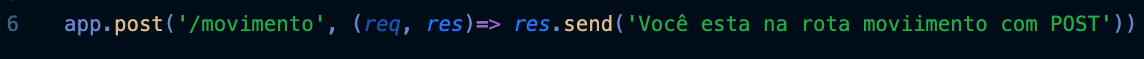
\includegraphics[width=115mm]{resources/aula4_12.png}\\
        \tiny{ Código no arquivo \textbf{movimentos.js}. \textbf{Fonte:} O autor}
     \end{center}   
      % \end{columns}
      Ao executar a aplicação notamos que nada muda....
    \end{frame}    
 %------------------------------------------------------------------------
 \subsection{Postman}
    \begin{frame}{Postman}
      %\begin{columns}[onlytextwidth]
        %\column{.5\textwidth}
 	O Postman é uma ferramenta que dá suporte à documentação das requisições feitas pela API. Ele possui ambiente para a documentação, execução de testes de APIs e requisições em geral.
        
       % \column{.5\textwidth}
         \begin{center}
    	
\includegraphics[width=85mm]{resources/aula4_13.png}\\
        \tiny{ Logo Postman. \textbf{Fonte:} POSTMAN, 2020}
     \end{center}   
      % \end{columns}
      Acesse \href{https://www.postman.com/}{https://www.postman.com/} e, faça o download da ferramenta.
    \end{frame}    
 %------------------------------------------------------------------------
    \begin{frame}{Postman - GUI}
      %\begin{columns}[onlytextwidth]
        %\column{.5\textwidth}
 	Aqui poderemos testar vários tipos de requisições feitas ao servidor.
        
       % \column{.5\textwidth}
         \begin{center}
    	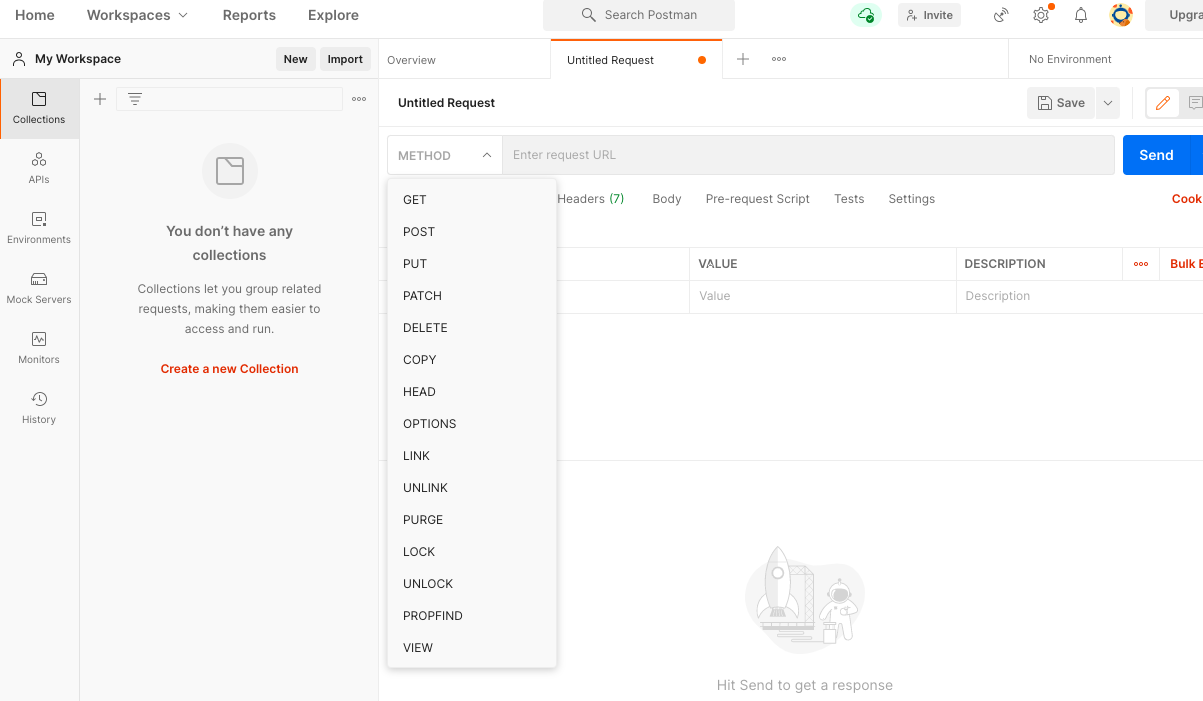
\includegraphics[width=95mm]{resources/aula4_14.png}\\
        \tiny{ Visual GUI Postman. \textbf{Fonte:} \cite{postman2022}.}
     \end{center}   
      % \end{columns}
    \end{frame}    
%-------------------------------------------
\section{Atividades}
\begin{frame}{Atividade}
Leia o material sobre functions, disponível em: 
\href{https://developer.mozilla.org/pt-BR/docs/Web/JavaScript/Reference/Functions}{Developers Mozila - Functions JS;}
Leia também: \href{https://developer.mozilla.org/pt-BR/docs/Web/JavaScript/Reference/Functions/Arrow_functions}{Developers Mozila - Arrow functions}.
\begin{itemize}
    \item 1. Desenvolva uma função, utilizando uma declaração ou expressão de função. Essa função deverá possuir dois parâmetros (valor, quantidade). A função deve mostrar no console a seguinte frase: “Cálculo: Preço: R\$ valor x quantidade. O total é: (valor*quantidade) ”.
    \item 2. Desenvolva novamente o exercício 1, utilizando Arrow Function. Utilize os mesmos parâmetros e retorne no console a mesma frase.
\end{itemize}
\end{frame}

\begin{frame}{Atividades}
Desenvolva os Exercícios:
\begin{itemize}
    \item 3. Desenvolva uma função chamada cambio, que receba um parâmetro chamado moeda e um parâmetro chamado valor. Dentro da função, retorne o resultado do valor em Reais.
    \item 4. Replique o exercício 3 utilizando Arrow Function.
\end{itemize}

\textit{Para todos os exercícios Não esqueça de mostrar o resultado no console!}


Envie como resposta apenas o código desenvolvido, não é necessário anexar arquivos

    
\end{frame}

%------------------------------------------------------------------------
\section{Referências}
\begin{frame}{Referências}%[allowframebreaks]
\small
\begin{center}
\tiny
\bibliographystyle{apalike}
\bibliography{ref_aula}
\end{center}
\end{frame}
  
\end{document}
